

\begin{figure}
    \begin{center}
        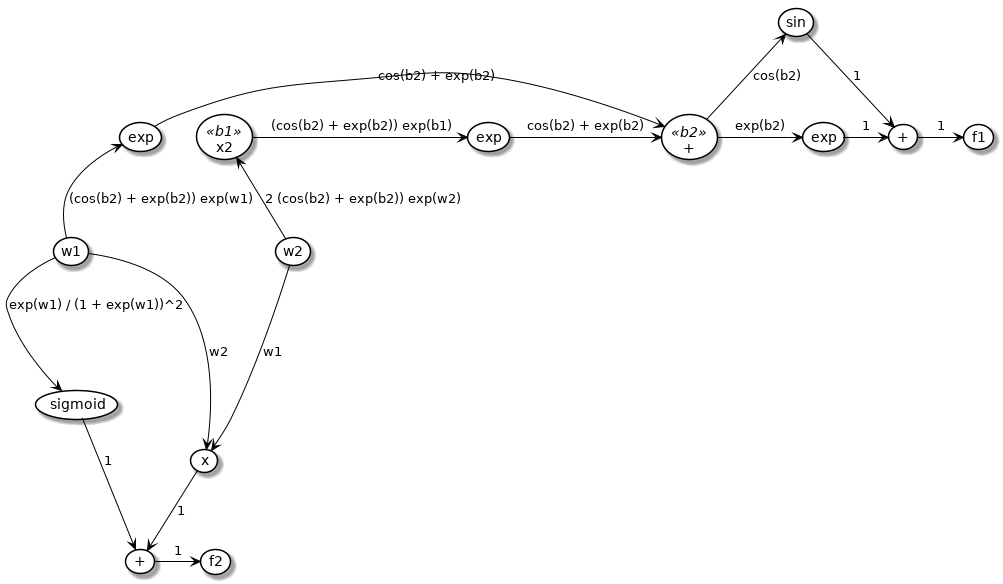
\includegraphics[width=.6\textwidth]{computation_graph_backward.png}
        \label{Backward gradient decent on $\vec{f}$}
    \end{center}
\end{figure}

Which in a more mathematical format give us:

\[
    \frac{\partial \vec{f}}{\partial \vec{w}} =
    \begin{bmatrix}
        ( \cos(e^{w_1} + e^{2 w_2}) + e^{e^{w_1} + e^{2 w_2}} ) e^{w_1}   &   2 ( \cos(e^{w_1} + e^{2 w_2}) + e^{e^{w_1} + e^{2 w_2}} ) e^{2 w_2} \\
        \frac{e^{w_1}}{(1 + e^{w_1})^2} + w_2                             &   w_1
    \end{bmatrix}
\]
